%% bare_conf.tex
%% V1.3
%% 2007/01/11
%% by Michael Shell
%% See:
%% http://www.michaelshell.org/
%% for current contact information.
%%
%% This is a skeleton file demonstrating the use of IEEEtran.cls
%% (requires IEEEtran.cls version 1.7 or later) with an IEEE conference paper.
%%
%% Support sites:
%% http://www.michaelshell.org/tex/ieeetran/
%% http://www.ctan.org/tex-archive/macros/latex/contrib/IEEEtran/
%% and
%% http://www.ieee.org/

%%*************************************************************************
%% Legal Notice:
%% This code is offered as-is without any warranty either expressed or
%% implied; without even the implied warranty of MERCHANTABILITY or
%% FITNESS FOR A PARTICULAR PURPOSE! 
%% User assumes all risk.
%% In no event shall IEEE or any contributor to this code be liable for
%% any damages or losses, including, but not limited to, incidental,
%% consequential, or any other damages, resulting from the use or misuse
%% of any information contained here.
%%
%% All comments are the opinions of their respective authors and are not
%% necessarily endorsed by the IEEE.
%%
%% This work is distributed under the LaTeX Project Public License (LPPL)
%% ( http://www.latex-project.org/ ) version 1.3, and may be freely used,
%% distributed and modified. A copy of the LPPL, version 1.3, is included
%% in the base LaTeX documentation of all distributions of LaTeX released
%% 2003/12/01 or later.
%% Retain all contribution notices and credits.
%% ** Modified files should be clearly indicated as such, including  **
%% ** renaming them and changing author support contact information. **
%%
%% File list of work: IEEEtran.cls, IEEEtran_HOWTO.pdf, bare_adv.tex,
%%                    bare_conf.tex, bare_jrnl.tex, bare_jrnl_compsoc.tex
%%*************************************************************************

% *** Authors should verify (and, if needed, correct) their LaTeX system  ***
% *** with the testflow diagnostic prior to trusting their LaTeX platform ***
% *** with production work. IEEE's font choices can trigger bugs that do  ***
% *** not appear when using other class files.                            ***
% The testflow support page is at:
% http://www.michaelshell.org/tex/testflow/



% Note that the a4paper option is mainly intended so that authors in
% countries using A4 can easily print to A4 and see how their papers will
% look in print - the typesetting of the document will not typically be
% affected with changes in paper size (but the bottom and side margins will).
% Use the testflow package mentioned above to verify correct handling of
% both paper sizes by the user's LaTeX system.
%
% Also note that the "draftcls" or "draftclsnofoot", not "draft", option
% should be used if it is desired that the figures are to be displayed in
% draft mode.
%
\documentclass[conference]{IEEEtran}
\usepackage{mathrsfs}
\usepackage{amsfonts}
\usepackage{mathtools}
\usepackage{amsbsy}
\usepackage[ruled,vlined]{algorithm2e}
\usepackage{accents}
\makeatletter
\newcommand{\ubar}[1]{\underaccent{\bar}{#1}}
\newcommand{\removelatexerror}{\let\@latex@error\@gobble}
\newcommand{\nosemic}{\renewcommand{\@endalgocfline}{\relax}}% Drop semi-colon ;
\newcommand{\dosemic}{\renewcommand{\@endalgocfline}{\algocf@endline}}% Reinstate semi-colon ;
\newcommand{\pushline}{\Indp}% Indent
\newcommand{\popline}{\Indm\dosemic}% Undent
\let\oldnl\nl% Store \nl in \oldnl
\newcommand{\nonl}{\renewcommand{\nl}{\let\nl\oldnl}}% Remove line number for one line	
\makeatother% Add the compsoc option for Computer Society conferences.


%
% If IEEEtran.cls has not been installed into the LaTeX system files,
% manually specify the path to it like:
% \documentclass[conference]{../sty/IEEEtran}





% Some very useful LaTeX packages include:
% (uncomment the ones you want to load)


% *** MISC UTILITY PACKAGES ***
%
%\usepackage{ifpdf}
% Heiko Oberdiek's ifpdf.sty is very useful if you need conditional
% compilation based on whether the output is pdf or dvi.
% usage:
% \ifpdf
%   % pdf code
% \else
%   % dvi code
% \fi
% The latest version of ifpdf.sty can be obtained from:
% http://www.ctan.org/tex-archive/macros/latex/contrib/oberdiek/
% Also, note that IEEEtran.cls V1.7 and later provides a builtin
% \ifCLASSINFOpdf conditional that works the same way.
% When switching from latex to pdflatex and vice-versa, the compiler may
% have to be run twice to clear warning/error messages.






% *** CITATION PACKAGES ***
%
%\usepackage{cite}
% cite.sty was written by Donald Arseneau
% V1.6 and later of IEEEtran pre-defines the format of the cite.sty package
% \cite{} output to follow that of IEEE. Loading the cite package will
% result in citation numbers being automatically sorted and properly
% "compressed/ranged". e.g., [1], [9], [2], [7], [5], [6] without using
% cite.sty will become [1], [2], [5]--[7], [9] using cite.sty. cite.sty's
% \cite will automatically add leading space, if needed. Use cite.sty's
% noadjust option (cite.sty V3.8 and later) if you want to turn this off.
% cite.sty is already installed on most LaTeX systems. Be sure and use
% version 4.0 (2003-05-27) and later if using hyperref.sty. cite.sty does
% not currently provide for hyperlinked citations.
% The latest version can be obtained at:
% http://www.ctan.org/tex-archive/macros/latex/contrib/cite/
% The documentation is contained in the cite.sty file itself.






% *** GRAPHICS RELATED PACKAGES ***
%
\ifCLASSINFOpdf
  % \usepackage[pdftex]{graphicx}
  % declare the path(s) where your graphic files are
  % \graphicspath{{../pdf/}{../jpeg/}}
  % and their extensions so you won't have to specify these with
  % every instance of \includegraphics
  % \DeclareGraphicsExtensions{.pdf,.jpeg,.png}
\else
  % or other class option (dvipsone, dvipdf, if not using dvips). graphicx
  % will default to the driver specified in the system graphics.cfg if no
  % driver is specified.
  % \usepackage[dvips]{graphicx}
  % declare the path(s) where your graphic files are
  % \graphicspath{{../eps/}}
  % and their extensions so you won't have to specify these with
  % every instance of \includegraphics
  % \DeclareGraphicsExtensions{.eps}
\fi
% graphicx was written by David Carlisle and Sebastian Rahtz. It is
% required if you want graphics, photos, etc. graphicx.sty is already
% installed on most LaTeX systems. The latest version and documentation can
% be obtained at: 
% http://www.ctan.org/tex-archive/macros/latex/required/graphics/
% Another good source of documentation is "Using Imported Graphics in
% LaTeX2e" by Keith Reckdahl which can be found as epslatex.ps or
% epslatex.pdf at: http://www.ctan.org/tex-archive/info/
%
% latex, and pdflatex in dvi mode, support graphics in encapsulated
% postscript (.eps) format. pdflatex in pdf mode supports graphics
% in .pdf, .jpeg, .png and .mps (metapost) formats. Users should ensure
% that all non-photo figures use a vector format (.eps, .pdf, .mps) and
% not a bitmapped formats (.jpeg, .png). IEEE frowns on bitmapped formats
% which can result in "jaggedy"/blurry rendering of lines and letters as
% well as large increases in file sizes.
%
% You can find documentation about the pdfTeX application at:
% http://www.tug.org/applications/pdftex





% *** MATH PACKAGES ***
%
%\usepackage[cmex10]{amsmath}
% A popular package from the American Mathematical Society that provides
% many useful and powerful commands for dealing with mathematics. If using
% it, be sure to load this package with the cmex10 option to ensure that
% only type 1 fonts will utilized at all point sizes. Without this option,
% it is possible that some math symbols, particularly those within
% footnotes, will be rendered in bitmap form which will result in a
% document that can not be IEEE Xplore compliant!
%
% Also, note that the amsmath package sets \interdisplaylinepenalty to 10000
% thus preventing page breaks from occurring within multiline equations. Use:
%\interdisplaylinepenalty=2500
% after loading amsmath to restore such page breaks as IEEEtran.cls normally
% does. amsmath.sty is already installed on most LaTeX systems. The latest
% version and documentation can be obtained at:
% http://www.ctan.org/tex-archive/macros/latex/required/amslatex/math/





% *** SPECIALIZED LIST PACKAGES ***
%
%\usepackage{algorithmic}
% algorithmic.sty was written by Peter Williams and Rogerio Brito. This
% package provides an algorithmic environment fo describing algorithms. You
% can use the algorithmic environment in-text or within a figure environment
% to provide for a floating algorithm. Do NOT use the algorithm floating
% environment provided by algorithm.sty (by the same authors) or
% algorithm2e.sty (by Christophe Fiorio) as IEEE does not use dedicated
% algorithm float types and packages that provide these will not provide
% correct IEEE style captions. The latest version and documentation of
% algorithmic.sty can be obtained at: http://www.ctan.org/tex-
% archive/macros/latex/contrib/algorithms/ There is also a support site at:
% http://algorithms.berlios.de/index.html Also of interest may be the
% (relatively newer and more customizable) algorithmicx.sty package by Szasz
% Janos: http://www.ctan.org/tex-archive/macros/latex/contrib/algorithmicx/




% *** ALIGNMENT PACKAGES ***
%
%\usepackage{array}
% Frank Mittelbach's and David Carlisle's array.sty patches and improves
% the standard LaTeX2e array and tabular environments to provide better
% appearance and additional user controls. As the default LaTeX2e table
% generation code is lacking to the point of almost being broken with
% respect to the quality of the end results, all users are strongly
% advised to use an enhanced (at the very least that provided by array.sty)
% set of table tools. array.sty is already installed on most systems. The
% latest version and documentation can be obtained at:
% http://www.ctan.org/tex-archive/macros/latex/required/tools/

%\usepackage{mdwmath}
%\usepackage{mdwtab}
% Also highly recommended is Mark Wooding's extremely powerful MDW tools,
% especially mdwmath.sty and mdwtab.sty which are used to format equations
% and tables, respectively. The MDWtools set is already installed on most
% LaTeX systems. The lastest version and documentation is available at:
% http://www.ctan.org/tex-archive/macros/latex/contrib/mdwtools/


% IEEEtran contains the IEEEeqnarray family of commands that can be used to
% generate multiline equations as well as matrices, tables, etc., of high
% quality.


%\usepackage{eqparbox}
% Also of notable interest is Scott Pakin's eqparbox package for creating
% (automatically sized) equal width boxes - aka "natural width parboxes".
% Available at:
% http://www.ctan.org/tex-archive/macros/latex/contrib/eqparbox/





% *** SUBFIGURE PACKAGES ***
%\usepackage[tight,footnotesize]{subfigure}
% subfigure.sty was written by Steven Douglas Cochran. This package makes it
% easy to put subfigures in your figures. e.g., "Figure 1a and 1b". For IEEE
% work, it is a good idea to load it with the tight package option to reduce
% the amount of white space around the subfigures. subfigure.sty is already
% installed on most LaTeX systems. The latest version and documentation can
% be obtained at:
% http://www.ctan.org/tex-archive/obsolete/macros/latex/contrib/subfigure/
% subfigure.sty has been superceeded by subfig.sty.



%\usepackage[caption=false]{caption}
%\usepackage[font=footnotesize]{subfig}
% subfig.sty, also written by Steven Douglas Cochran, is the modern
% replacement for subfigure.sty. However, subfig.sty requires and
% automatically loads Axel Sommerfeldt's caption.sty which will override
% IEEEtran.cls handling of captions and this will result in nonIEEE style
% figure/table captions. To prevent this problem, be sure and preload
% caption.sty with its "caption=false" package option. This is will preserve
% IEEEtran.cls handing of captions. Version 1.3 (2005/06/28) and later 
% (recommended due to many improvements over 1.2) of subfig.sty supports
% the caption=false option directly:
%\usepackage[caption=false,font=footnotesize]{subfig}
%
% The latest version and documentation can be obtained at:
% http://www.ctan.org/tex-archive/macros/latex/contrib/subfig/
% The latest version and documentation of caption.sty can be obtained at:
% http://www.ctan.org/tex-archive/macros/latex/contrib/caption/




% *** FLOAT PACKAGES ***
%
%\usepackage{fixltx2e}
% fixltx2e, the successor to the earlier fix2col.sty, was written by
% Frank Mittelbach and David Carlisle. This package corrects a few problems
% in the LaTeX2e kernel, the most notable of which is that in current
% LaTeX2e releases, the ordering of single and double column floats is not
% guaranteed to be preserved. Thus, an unpatched LaTeX2e can allow a
% single column figure to be placed prior to an earlier double column
% figure. The latest version and documentation can be found at:
% http://www.ctan.org/tex-archive/macros/latex/base/



%\usepackage{stfloats}
% stfloats.sty was written by Sigitas Tolusis. This package gives LaTeX2e
% the ability to do double column floats at the bottom of the page as well
% as the top. (e.g., "\begin{figure*}[!b]" is not normally possible in
% LaTeX2e). It also provides a command:
%\fnbelowfloat
% to enable the placement of footnotes below bottom floats (the standard
% LaTeX2e kernel puts them above bottom floats). This is an invasive package
% which rewrites many portions of the LaTeX2e float routines. It may not work
% with other packages that modify the LaTeX2e float routines. The latest
% version and documentation can be obtained at:
% http://www.ctan.org/tex-archive/macros/latex/contrib/sttools/
% Documentation is contained in the stfloats.sty comments as well as in the
% presfull.pdf file. Do not use the stfloats baselinefloat ability as IEEE
% does not allow \baselineskip to stretch. Authors submitting work to the
% IEEE should note that IEEE rarely uses double column equations and
% that authors should try to avoid such use. Do not be tempted to use the
% cuted.sty or midfloat.sty packages (also by Sigitas Tolusis) as IEEE does
% not format its papers in such ways.





% *** PDF, URL AND HYPERLINK PACKAGES ***
%
%\usepackage{url}
% url.sty was written by Donald Arseneau. It provides better support for
% handling and breaking URLs. url.sty is already installed on most LaTeX
% systems. The latest version can be obtained at:
% http://www.ctan.org/tex-archive/macros/latex/contrib/misc/
% Read the url.sty source comments for usage information. Basically,
% \url{my_url_here}.





% *** Do not adjust lengths that control margins, column widths, etc. ***
% *** Do not use packages that alter fonts (such as pslatex).         ***
% There should be no need to do such things with IEEEtran.cls V1.6 and later.
% (Unless specifically asked to do so by the journal or conference you plan
% to submit to, of course. )


% correct bad hyphenation here
\hyphenation{op-tical net-works semi-conduc-tor}


\begin{document}
%
% paper title
% can use linebreaks \\ within to get better formatting as desired
\title{A Comparative Analysis of Value Function Approximation Approaches in Reinforcement Learning}


% author names and affiliations
% use a multiple column layout for up to three different
% affiliations
\author{\IEEEauthorblockN{Zhiwei Han}
\IEEEauthorblockA{Faculty of Electrical Engineering and Information Technology\\
Technical University of Munich\\
Arcisstr. 21, Munich, 80333\\
Email: hanzw356255531@icloud.com}
}

% conference papers do not typically use \thanks and this command
% is locked out in conference mode. If really needed, such as for
% the acknowledgment of grants, issue a \IEEEoverridecommandlockouts
% after \documentclass

% for over three affiliations, or if they all won't fit within the width
% of the page, use this alternative format:
% 
%\author{\IEEEauthorblockN{Michael Shell\IEEEauthorrefmark{1},
%Homer Simpson\IEEEauthorrefmark{2},
%James Kirk\IEEEauthorrefmark{3}, 
%Montgomery Scott\IEEEauthorrefmark{3} and
%Eldon Tyrell\IEEEauthorrefmark{4}}
%\IEEEauthorblockA{\IEEEauthorrefmark{1}School of Electrical and Computer Engineering\\
%Georgia Institute of Technology,
%Atlanta, Georgia 30332--0250\\ Email: see http://www.michaelshell.org/contact.html}
%\IEEEauthorblockA{\IEEEauthorrefmark{2}Twentieth Century Fox, Springfield, USA\\
%Email: homer@thesimpsons.com}
%\IEEEauthorblockA{\IEEEauthorrefmark{3}Starfleet Academy, San Francisco, California 96678-2391\\
%Telephone: (800) 555--1212, Fax: (888) 555--1212}
%\IEEEauthorblockA{\IEEEauthorrefmark{4}Tyrell Inc., 123 Replicant Street, Los Angeles, California 90210--4321}}




% use for special paper notices
%\IEEEspecialpapernotice{(Invited Paper)}




% make the title area
\maketitle

% The goal of reinforcement learning is to obtain an efficient and universal learning algorithm, which is possible to learn from experimental knowledge and able to react by given enviromental information.
% Temporal-Difference is a traditional and effi
% GQ($\lambda$) is a variation of classic Q-Learning method which applied the gradient decent method to iteratively update the Q-Functions directly(tabularwise algorithm) to minimize the Mean-Squre Projected Bellman Error. This 
% In GQ($\lambda$) and RO-GQ($\lambda$), 
% Besides the Framework, the significant difference between the comparised algorithm is the 
% Even with the lineraly growing of state or action number, the computational expense increases exponentially. Hence, a sparse presentation of Q-Functions would be one smart solution to this kind of problem. 
\begin{abstract}
%\boldmath
In this paper, a comparison of three value function approximation based reinforcement learning algorithms is presented to evaluate their performance on solving continuous state space control problem. They are GQ($\lambda$), $\ell1$ norm regularized off-policy TD($\lambda$) and online selective kernel-based TD($\lambda$). For convenience, these algorithms will be called GQ($\lambda$), RO-TD($\lambda$) and OSK-TD($\lambda$) in rest of the paper. The comparison standard concentrates mainly on the total reward, convergence and efficiency of the algorithms. The classic TD($\lambda$) framework Q-Learning is applied and adapted by compared algorithms in parameter learning. Note, other RL framework choice like Sarsa($\lambda$) could also be possible, but won't be discussed here. GQ($\lambda$), which minimize the mean-squre projected Bellman error(MSPBE) with gradient descend, is a very powerful and straightforward learning method under small scale or well-defined discrete space setting condition. However, because of the curve of dimensionality, the algorithm could be less computational efficient as the increasing number of state. To overcome this issue, one $\ell1$ regularity term was inserted to the objective function in RO-GQ($\lambda$) algorithm. The sparsity generated in the learned parameters helps significantly reduce the computational complexity of RO-GQ($\lambda$) and therefore it has a better performance in these problems. Alternatively, OSK-TD($\lambda$) provides another solution for sparsification, which is less computational complex and can be runned online. OSK-TD includes two procedures, a dictionary consists of feature vector is online generated and refreshed with a criteria for whether and how to add a new feature in dictionary. In the second step, a kernel selective function $\beta$(s) selects the best matched feature vector in dictionary for the selective kernel-based Q-function representation. 
\end{abstract}
% IEEEtran.cls defaults to using nonbold math in the Abstract.
% This preserves the distinction between vectors and scalars. However,
% if the journal you are submitting to favors bold math in the abstract,
% then you can use LaTeX's standard command \boldmath at the very start
% of the abstract to achieve this. Many IEEE journals frown on math
% in the abstract anyway.

% Note that keywords are not normally used for peerreview papers.
\begin{IEEEkeywords}
reinforcement learning, Q-Learning, function approximation, sparsification, slective kernel-based value function
\end{IEEEkeywords}






% For peer review papers, you can put extra information on the cover
% page as needed:
% \ifCLASSOPTIONpeerreview
% \begin{center} \bfseries EDICS Category: 3-BBND \end{center}
% \fi
%
% For peerreview papers, this IEEEtran command inserts a page break and
% creates the second title. It will be ignored for other modes.
\IEEEpeerreviewmaketitle



\section{Introduction}
Reinforecement learning (RL) approaches to classic predict and control problems base on dynamic programming (DP) and markov decision process (MDP) model, which proofed to be useful but computational expensive in high dimensional case. Sutton and Barto [1] proposed temporal difference (TD) learning framework and its variations as the extension of DP. One of its nice properties is the combination with value function approximation and it makes the algorithm possible to learn from complicated learning tasks.\\


But there are still two problems about value function approximation mainteined unsovled. In practical large scale problems, smart value function approximation strategy is alwags required to reduce the computational complexity because large scale RL problems e.g. Go within continous/action spaces suffer from the curse of dimensionality, which means the computational complexity increases exponentially with growing number of states and actions. This problem arises as a main subproblem in RL and is generally considered as the most important step in RL algorithm development. There are serveral value function approximation techniques developed in recent researches, e.g. linear function approximation \cite{sutton1998reinforcement} \cite{tsitsiklis1997analysis}, regression tree \cite{ernst2005tree} and kernel-method \cite{xu2007kernel}\cite{ormoneit2002kernel}, which can deal with a specific set of problems. More generally, after deep learning \cite{lecun2015deep} concept and deep neural network were introduced into RL, the perforemance has been significantly improved since Alpha Go of Deep Mind, a company owned by Google, beated one of the best human Go players, Lee Sedong. Furthermore, the learning agent equipped with deep Q-network (DQN) \cite{mnih2015human} based Q function Approximator was also turned out to be smarter than human player in some Atri-games. Regularization could be another solution to this problem, it plays not only an important role in preventing overfitting and is also considered as an ideal feature selection technique for in algorithms with value function approximation thanks to the sparsity generated by $\ell1$ norm reguarization\cite{kolter2009regularization} \cite{liu2012regularized}. In this paper, the tabular algorithm RO-TD($\lambda$) with $\ell1$ norm reguarization is compared with the algorithm OSK-TD($\lambda$) \cite{chen2013online}, which equipped with another feature selection strategy, in term of the efficency of sparsification.\\

Another widely concerned issure is convergence of the value function approximation. As Tsitsiklis \cite{tsitsiklis1997analysis} pointed out that even though the linear value function approximation converges in most online learning problem setting, but an algorithm could still diverge if either of the conditions is not satisfied, when a off-line learning is perform, because states are sampled from distributions independent of the dynamics of the Markov chain of interst, or a nonlinear value function approximation is used. We will also point out this kind of view later in the experiment. It's a servere problem in RL application, however, because of the great needs, value function approximation was still applied in many off-line TD algorithms like Q-learning at that time while ignoring the potential risk of divergent value function approximation. Sutton \cite{sutton1998reinforcement}\cite{sutton2009fast} solved off-line learning problem of off-policy learning by introducing a new object function, \textit{mean-squre projected Bellman error} (\textup{MSPBE}) and performing stochastic gradient mehtod an it.\\

In this paper, we consider up-to-date algorithms GQ($\lambda$) \cite{maei2010gq}, RO-GQ($\lambda$) \cite{liu2012regularized} based on the traditional tabular algorithm framework (without value function approximation), kernel-based feature selective algorithm OSK-TD($\lambda$) \cite{chen2013online} and their comparison. The rest of this paper is organized as flollows. In Section \uppercase\expandafter{\romannumeral2}, an introduction on MDPs as well as the TD learning framework is given. \uppercase\expandafter{\romannumeral3} presents the used techniques in the algorithms to be compared. An algorithmetic introduction and comparison between three algorithm is proposed in the section \uppercase\expandafter{\romannumeral4}. And in section \uppercase\expandafter{\romannumeral5} the experimental result on the classic RL problem settings Mountain Car and Carto Car are provided to visulization the effectiveness of compared algorithm. At the \uppercase\expandafter{\romannumeral6} section gives a conclussion and future work.\\

\section{RL and Background}
\subsection{Framework and Notation}
In this paper, we consider infinite markov decision process with discrete state space $\mathcal{S}$ and discrete action space $\mathcal{A}$. A  MDP can be defined as tuple ($\mathcal{S}$, $\mathcal{A}$, $\mathcal{P}$, $r$, $\gamma$), where $\mathcal{P}$ represents the transition probability matrix and it is also defined as the one-step dynamics of enviroment by given state and action. \cite{sutton1998reinforcement} Given any state and action, $s$ and $a$, the probability of each possible state transition to next state $s'$, is a function $Pr:\mathcal{S}\times\mathcal{S}\times\mathcal{A}\mapsto[0, 1]$
\begin{equation}
  p(s'|s, a)=Pr\{S_{t+1}=s'|S_t=s,A_t=a\}
\end{equation}


Similarly, with any current state and action, $s$ and $a$, and after taking action a the agent reaches the next state $s'$, the expected value of the next reward of tuple ($s$, $a$, $s'$) is a function $r:\mathcal{S}\times\mathcal{A}\times\mathcal{S}\mapsto\mathbb{R}$ and $\gamma\in(0, 1)$ is the discount factor.
\begin{equation}
  r(s, s', a)=\mathbb{E}[R_{t+1}|S_t=s,A_t=a, S_{t+1}=s']
\end{equation}

In RL, main task is either directly to find a convergent value function through like dynamic programming etc., or indirectly approximate a value function (action-value function) through linear value function approximation etc.. A value function maps from each state to a number representation of value function obtained if a policy is exactly followed. Policy can also be analysed and evaluated according its sum of discounted value function. More formally, 
\begin{equation}
V^{\pi}(s) = \mathbb{E}[\sum_{t=0}^{\inf}\gamma^{t}r_{t+1}]
\end{equation}
\begin{equation}
P^{\pi}(s, s') = \sum_{a\in\mathcal{A}}\pi(s, a)P(s'|s,a)
\end{equation}
\begin{equation}
R^{\pi}(s) = \sum_{a\in\mathcal{A}}\sum_{s'\in\mathcal{S}}\pi(s, a)p(s'|s, a)r(s, a, s')
\end{equation}

If $V^{\pi}$, $R^{\pi}$ are vectorized with length $|\mathcal{S}|$ and the dimension of $P^\pi$ is $|\mathcal{S}|\times|\mathcal{S}|$, so the famous $Bellman$ $Equation$ can be written in form,
\begin{equation}
V^\pi=TV^\pi=R^\pi + \gamma P^\pi V^\pi
\end{equation}
, where $T$ is the Bellman operator and $V^\pi$ is the fix point of Bellman operation.\\ 

In rest of this paper, value function is replaced of action-value function, which maps each state and action, instead of only state, to a number representation, as we mainly focus on control problem.

\subsection{Tabular version of Q($\lambda$)}
The basic idea of temporal difference learning is looking back to the previous state, and correcting the previous value or action-value function with experience (Bellman Error). The update of value function is defined as following,
\begin{equation}
  V(s_t) = V(s_t) + \alpha \delta(s_t)
\end{equation}
, where $\alpha$ is the learning rate and $\delta$ is the Bellman error, which defined as
\begin{equation}
  \delta(s_t) = R_{t+1} + \gamma V(s_{t+1}) - V(s_t)
\end{equation}

As one of the most important extension of TD algorithm, the off-policy learning procedure Q-Learning\cite{watkins1992q}, whose update form is,
\begin{equation}
  \begin{split}
    &Q(s_t, a_t) = Q(s_t, a_t) + \alpha [R_{t+1} + \\
    &\gamma \max_{a\in A}Q(s_{t+1}, a) - Q(s_t, a_t)]\\
  \end{split}  
\end{equation}
, directly approximates $Q^*$, the optimal action-value function, independent of the policy being followed.\\

Based on the TD method, eligibility keeps track on several prior states and how the action-value function should be updated when a new observation is revceived. More precisely, eligibility is a temporal record of occured events e.g. states or actions, and propagates the attenuated TD error back then finally updates the parameters of the previous states. The famous combinations of Q-learning and eligibility trace are Watkins’s Q($\lambda$) \cite{watkins1992q} and Peng’s Q($\lambda$) \cite{peng1996incremental} for different update rules of eligibility trace. \\

The tabular version of Q($\lambda$) is a special case of linear action-value function approximation based Q($\lambda$). With a sparse feature vector $\phi$ for a given state and action pair, only one entry in learned parameter vector $\theta$ is going to be chosen when doing a vector multiplication. And this entry serves exactly as the Q-Function for the given feature vector.
\begin{equation}
  Q(s, a) = \theta^\top  \phi(s, a)
\end{equation}

So a vectorise and parallel version implementation of traditional Q($\lambda$) is possible and the update rule of TD error $\delta$ and eligibility trace $e$ in form of Q-Learning from backward view is following,
\begin{equation}
  \delta_t = R + \gamma \max_a \theta^\top  \phi(s_{t+1}, a) - \theta^\top  \phi(s_t, a_t)
\end{equation}
\begin{equation}
  e_t = \alpha \lambda e_t + \phi_t
\end{equation}

Note, here we assume the transitions between states are ergodic, for a nonergodic case, replacing trace technique will be helpful. Finally, the update rule of parameter $\theta$ is given as following,
\begin{equation}
  \theta_{t+1} = \theta_t + \alpha \delta e
\end{equation}


\section{GQ($\lambda$)}
One natural RL approach to learning task can be turned into an optimization problem, where we seek to minimize a predefined objective function by updating its parameter θ. The objective function should reflect how well (or how badly) the value function is approximated and ideally it can be written in form of weighted square norm as \textit{mean square error} (\textup{MSE}),
\begin{equation}
    \textup{MSE}(\theta):=||V_\theta-V||^2_D, 
\end{equation}
where $D$ is a weight matrix, whose diagnal entries are a weight scalars $\{d_1, d_2,..., d_n\}$.
In TD methods, the idea is to replace the \textup{MSE} with \textit{mean-square Bellman error} (\textup{MSBE}) \cite{baird1995residual} \cite{baird1999reinforcement} how closely the approximate value function satisfies the Bellman equation.
\begin{equation}
    \textup{MSBE}(\theta):=||V_\theta-TV_\theta||^2_D.
\end{equation}
This is the objective function used by the most important prior effort to develop gradient-descent algorithms. But the prior algorithms like TD, LSTD, and GTD don't sufficiently converge to the minimum of \textup{MSE} as Bellman operator typically is irrespective of  value function approximation structure. Hence, it is not be able to represent value function approximation for any $\theta$, although it follows the dynamics of Markov Decision Process (MDP).\\
By introducing the project operator in linear approximation architecture
\begin{equation}
  \Pi = \Phi(\Phi^\top D\Phi)^{-1}\Phi^\top D ,
\end{equation}
which can project any value function to the subspace of linear architecture, we obtain the most accurate function approximator of $v$ in the subspace of linear architecture. In other words
\begin{equation}
  \Pi v = V_\theta \ \textup{where}\ \theta = \arg \min_\theta||V_\theta-v||^2_D.
\end{equation}
After the projection operator was introduced, all algorithms mentioned before find or converge to a fixpoint of the composed projection and Bellman operators, which is a value of $\theta^*$ such that
\begin{equation}
  V_{\theta^*} = \Pi TV_{\theta^*}
\end{equation}
and named as TD fixpoint. The objective function used in this paper is very similar to the \textit{mean-square projected Bellman error} (\textup{MSPBE})
\begin{equation} 
  \textup{MSPBE}(\theta)=||V_{\theta}-\Pi TV_{\theta}||^2_D,
\end{equation}
deviated from this fixpoint.\\

As an extension version of the TDC \cite{sutton2009fast}, GQ($\lambda$) minimizes its objective function by iteratively updating the parameter with eligibility traces and multi-step reward. Its objective function is a $\lambda$-step weighted version of the \textup{MSPBE} and denoted as 
\begin{equation}
\begin{split}
  &J(\theta) \\{}
  &= \|Q_\theta - \Pi\mathnormal{T}_\pi^{\lambda\beta}Q_\theta\|^2_D\\
  &=(T_\pi^{\lambda\beta}Q_\theta - Q_\theta)^\top \Pi^\top D\Pi(T_\pi^{\lambda\beta}Q_\theta - Q_\theta)\\
  &=(\Phi^\top D(T_\pi^{\lambda\beta}Q_\theta - Q_\theta))^\top (\Phi^\top D\Phi)^{-1}\Phi^\top D(T_\pi^{\lambda\beta}Q_\theta - Q_\theta)\\
  &=\mathbb{E}_\pi[\delta^{\lambda\beta} \phi]^\top \mathbb{E}[\phi\phi^\top ]^{-1}\mathbb{E}[\delta^{\lambda\beta} \phi],
  \end{split}
\end{equation}
at the fix point $\theta$ \cite{sutton2009fast} \cite{maei2010gq}, where the identity $\Pi^\top D\Pi=D\top\Phi(\Phi^\top D\Phi)^{-1}\Phi^\top D$ is used and $g^{\lambda \beta\rho}$, $\delta^{\lambda\beta\rho}$ stand for $\lambda$-return and $\lambda$-step TD error, respectively,
\begin{equation}  
  \begin{split}
    & g^{\lambda\beta\rho}_t=r_{t+1}+\beta_{t+1}e_{t+1}\\
    &+(1-\beta_{t+1})[(1-\lambda_{t+1})\theta^{\top}{\bar{\phi}}_{t+1}+\lambda_{t+1}\rho_{t+1}g_{t+1}^{\lambda\beta\rho}]\\
    &\textup{and}\\
    &\delta^{\lambda\beta\rho}_t=g^{\lambda\beta\rho}_t-\theta^{\top} \phi_t,
  \end{split}
\end{equation}
and, 
\begin{equation}
\bar{\phi}_t=\sum_a \pi(s_t, a)\phi(s_t, a)\ \textup{and} \ \rho_t = \frac{\pi(s_t, a)}{b(s_t, a)}
\end{equation}

After taking the negative gradient of objective function as the optimization direction,
\begin{equation}
\begin{split}
  &-\frac{1}{2}\nabla MSPBE(\theta) =-\frac{1}{2}\nabla J(\theta) \\
  &= -\mathbb{E}_b[(\nabla g^{\lambda \beta\rho} - \phi) \phi^\top ]\mathbb{E}_b[\phi\phi^\top ]^{-1}\mathbb{E}_b[\delta^{\lambda\beta\rho}\phi]\\
  &\approx \mathbb{E}[\delta^{\lambda\beta\rho}\phi]-\mathbb{E}_b[\nabla g^{\lambda \beta\rho}\phi^\top ]\omega,
  \end{split}
\end{equation}
where a second modifiable parameter $\omega\in\mathbb{R}^n$ is used to avoid caculating the inverse matrix and double sampling   \cite{sutton1998reinforcement},
\begin{equation}
  \omega\approx \mathbb{E}_b[\phi^\top \phi]^{-1}\mathbb{E}_b[\delta^{\lambda\beta\rho}\phi],
\end{equation}
finally the forward and backward view update of $GQ(\lambda)$ are given as the proof in \cite{maei2010gq}
\begin{equation}
\begin{split}
  &\textup{Forward:}\\
  &\theta_{t+1}=\theta{t}+\alpha_{\theta, t}\bigg(\delta^{\lambda\beta\rho}_t\phi_t-\nabla g^{\lambda\beta\rho}_t\phi_t^\top\omega_t\bigg)\\
  &\omega_{t+1}=\omega_t+\alpha_{\omega, t}\bigg(\delta^{\lambda\beta\rho}_t-\omega_t^\top\phi_t\bigg)\phi_t\\
  &\textup{Backward:}\\
  &\theta_{t+1}=\theta_t+\alpha_{\theta, t}[\delta_te_t-\kappa_{t+1}({e_t}\top \omega_{t}){\bar{\phi}}_{t+1}]\\
  &\omega_{t+1}=\omega_{t}+\alpha_{\omega, t}[\delta_te_t-(\omega^\top\phi_t)\phi_t],
\end{split}
\end{equation}
where
\begin{equation}
\kappa_t=(1-\beta_t)(1-\lambda_t) \ \textup{and} \ e_t=\phi_t+(1-\beta_t)\lambda_t\rho_t\phi_{t-1}.
\end{equation}
Then we give the pseudocode of GQ($\lambda$)\\
{
\LinesNumbered
\removelatexerror% Nullify \@latex@error
\begin{algorithm}[H]
	\textup{Initialization $\pmb{\theta}$ arbitrarily and $\pmb{\omega}$ = 0} \\
	\Repeat({ (for each episode)}){}{
		\textup{Initialize $\pmb{e}$ = 0}\\
		\textup{$S\leftarrow$ initial state of episode}\\
		\Repeat({(for each step of episode)}){\textup{$S^{'}$ is terminal}}{
	  		\textup{$A\leftarrow$ action selected by policy $b$ in state $S$}\\
	  		\textup{Take action}\ A,\ \textup{observe next state,}\ $S^{'}$\\
	  		$\bar{\phi}\leftarrow 0$\\ 
	  \textup{For all $a \in \mathcal{A}(s)$:$\bar{\phi}\leftarrow\bar{\phi}+\pi(S^{'}, a)\phi(S^{'}, a)$}\\
	  $\rho = \frac{\pi(S, A)}{b(S, A)}$\\
	  	\textup{GQlearn($\phi(S, A)$, $\bar{\phi}$, $\lambda(S^{'})$,$ \gamma(S^{'})$, $r(S, A, S^{'})$, $\rho$, $I(S)$)}\\
	  $S\leftarrow S^{'}$
  	}
  	}
	\caption{GQ($\lambda$)}
\end{algorithm}
}
{
\LinesNumbered
\removelatexerror% Nullify \@latex@error
\begin{algorithm}[H]
$\delta\leftarrow R+\lambda \pmb{\theta}^{\top} \bar{\phi}-\pmb{\theta}^{\top}\phi$\\
$\pmb{e}\leftarrow \rho \pmb{e} + I \phi$\\
$\pmb{\theta} \leftarrow \pmb{\theta}+ \alpha (\delta \pmb{e} -\gamma(1-\lambda)(\omega^{\top}\pmb{e})\bar{\phi}))$\\
$\pmb{\omega}\leftarrow\pmb{\omega}+\alpha\eta(\delta\pmb{e}-(\pmb{\omega}^{\top}\phi)\phi)$\\
$\pmb{e}\leftarrow\gamma\lambda\pmb{e}$\\
 \caption{GQlearn($\phi,\bar{\phi},\lambda,\gamma, R, \rho, I$)}
\end{algorithm}
}
\section{RO-GQ($\lambda$)}
RO-GQ($\lambda$) is a novel $\ell1$ regularized off-policy convergent TD-learning algorithm with low computational complexity, which is able to learn sparse representations of value function by performing $\ell1$ regularization in learning procedure. The algorithmic framework of RO-TD integrates two key schemas: off-policy convergent gradient TD methods and a convex-concave saddle-point formulation of non-smooth convex optimization ($\ell1$ regularization term in objective function, which enables first-order solvers and feature selection using online convex regularization. \\

Due to the special objective function used in RO-GQ($\lambda$), we present here the mathematical background needed by optimization procedure.
\subsection{Proximal Gradient Method}
Minimization of a composite objective function is useful in enforcing various structure , such as sparsity in case of $\ell1$ regularization on machine learning task. As well known property, $\ell1$ regularization is able to generate sparse representation optimization problem but can also lead to not-differentiability of objective function. Here we introduce proximal gradient method\cite{sra2012optimization}, which can be shown to be an efficient solution to non-differentiable convex problem caused by subdifferential of $\ell1$ regularization.\\
The basic form of proximal mapping associated with a convex function $h$ is defined as:
\begin{equation}
	prox_h(x)=\arg\min_{u}(h(u)+\frac{1}{2}||u-x||^2)l
\end{equation}
In case of $\ell1$ regularity term in objective function, which can be written in its general form $h(x)=\rho||x||_1(\rho > 0)$, the proximal operator is turned out to be a entry-wise soft-threshold operator denoted as $S_\rho(\cdot)$ and we obtain:
\begin{equation}
	\begin{split}
		&prox_h(x)_i\\
		&=S_\rho(x_i)\\
		&=max(x_i-\rho,0)-max(-x_i-\rho, 0),
	\end{split}
\end{equation}
where $i$ is the index and $\rho$ is the threshold. When the optimization problem is 
\begin{equation}
	x^*=\arg\min_{x\in\mathcal{X}}(f(x)+h(x)),
\end{equation}
where $f(x)$ is a convex and differentiable loss function and $h(x)$ is a convex but non-differentiable regularization term. After performing proximal gradient method, the iterative update of $x$ is
\begin{equation}
	x_{t+1}=prox_{\alpha_t h}(x_t-\alpha_t \nabla f(x_t)).
\end{equation}
where $\alpha_t$ is a step-size factor. And meanwhile it's also cheap for computing.
\subsection{Convex-concave Saddle-Point First Order Algorithm}
Another novel idea of RO-GQ($\lambda$) is a convex-concave saddle-point representation for regularized TD learning. A convex-concave saddle-point problem can be described as \cite{sra2012optimization}
\begin{equation}
	SadVal=\inf_{x\in\mathcal{X}}\sup_{y\in\mathcal{{Y}}}\phi(x,y),
\end{equation}
where $x\in\mathcal{X}, y\in\mathcal{Y}$ are non-empty closed convex sets and a continuous convex cost function $\phi(x, y)$ is convex in variable $x\in\mathcal{X}$ and concave in variable $y\in\mathcal{Y}$. By definition, solutions to convex-concave saddle-point problem (31) ($x^*,y^*$) should be in form of $\phi(x, y^*)\geq\phi(x^*, y^*)\geq\phi(x^*, y)$ for every $x\in\mathcal{X}$ and $y\in\mathcal{Y}$. The problem can also be written in form of primal-dual pair 
\begin{equation}
  \begin{split}
    &Opt(P)=\min_{x\in\mathcal{X}}\bar{\phi}(x),\ \bar{\phi}(x)=\sup_{y\in\mathcal{Y}}\phi(x, y)\\
    &Opt(D)=\max_{y\in\mathcal{Y}}\underset{\bar{}}{\phi}(y),\ \underset{\bar{}}{\phi}(y)=\inf_{x\in\mathcal{Y}}\phi(x, y).
  \end{split}
\end{equation}

$\phi$ possesses saddle-points if and only if optimization problem $P$ and $D$ have the equal optimal values or equivalently,
\begin{equation}
  Opt(P) = Opt(D).
\end{equation}

This property could be particularly helpful when solving, for example, a minimization problem which aims to minimize a well structured subdifferential convex objective function $\bar{\phi}(x) = \sup_{y\in\mathcal{Y}}\phi(x, y)$ over $x$, which is not solvable to many convex optimization techniques, where smoothness is required. By applying this property it can be converted to a dual maximization problem over $y$, whose objective function is a differentiable convex function $\underset{\bar{}}{\phi}(y)=\inf_{x\in\mathcal{X}}\phi(x, y)$. Therefore, convex-concave saddle-point approach is a possible solution for $\ell1$ norm problem.
\subsection{Objective Function}
Regarding the TDC algorithm \cite{sutton2009fast},whose update is
\begin{equation}
			\theta_{t+1} = \theta_{t}+\alpha_{t}\delta_t\phi_t -\alpha\gamma\phi_{t}^{'}(\phi_t^\top\omega_{t}),
\end{equation} 
where
\begin{equation} 
	\omega_{t+1}=\omega_{t}+\beta_{t}(\delta_{t}-\phi_{t}^\top\omega_{t})\phi_t,
\end{equation}
we obtain its generalization by combining it with eligibility trace and off-line learning
\begin{equation}
			\theta_{t+1} = \theta_{t}+\alpha_{t}[\delta_te_t -\gamma(1-\gamma)\omega_t^\top e_t\bar{\phi}_{t+1}],
\end{equation} 
where
\begin{equation} 
	\omega_{t+1}=\omega_{t}+\beta_{t}(\delta_{t}e_t-\omega_{t}\phi_{t}\phi_t).
\end{equation}

we combine the two iterations and reformulate it in one iterative equation as following,
\begin{equation}
	x_{t+1} = x_t-\alpha_t(A_tx_t-b_t),	
\end{equation}
where
\begin{equation}
\begin{split}
	&A_t = 	\begin{bmatrix} 
				\eta\phi_t\phi_t^\top & \eta e_t (\phi_t-\gamma\bar{\phi}_{t+1})^\top \\ 
				\gamma(1-\gamma)\bar{\phi}_{t+1}e_t^\top & e_t(\phi_t-\gamma\bar{\phi}_{t+1})^\top 
			\end{bmatrix},\\
	&b_t=\begin{bmatrix}\eta r_t e_t \\ r_te_t \end{bmatrix},\ \ \ \  x_t=\begin{bmatrix} \omega_t \\ \theta_t\end{bmatrix}.
\end{split}
\end{equation}
Thus, its one-step linear equation
\begin{equation}
	Ax = b,
\end{equation}
should be satisfied where matrix $A, x$ can be derived by taking its expectation alone the infinite episode, which equal to
\begin{equation}
	A = \mathbb{E}_t[A_t(\phi_t, \phi_t^{'})],\ \ b = \mathbb{E}_t[b_t(\phi_t, r_t)],\ \ x=\begin{bmatrix} \omega \\ \theta\end{bmatrix}.
\end{equation}

Before describing objective function, there are still some concerns from the perspective of convex optimization and reinforcement learning. First, $A$ is neither positive definite or symmetric, hence the convexity of objective function, which required by usual optimization algorithm, can not be guaranteed. Second concern is we do not have any knowledge about $A, b$, they must be separable within the objective function so that it can be approximated by sampling (stochastically solvable). Furthermore, to avoid double sampling we should ensure no Bellman residual or its derivative involved in objective function as double sampling is a necessary method for getting unbiased estimator where Bellman residual is included within objective function. Consequently, based all the listed limits and requirement of objective functions above, we finally present the regularized objective function as
\begin{equation}
	L(x)=||Ax-b||_m+h(x),
\end{equation}
where $m$ is a conjugate number.
\subsection{RO-GQ($\lambda$) Design}
By definition a conjugate norm can be written as \cite{sra2012optimization}
\begin{equation}
	||\xi||_* = \max_{x}\big\{\big<\xi, x\big>:||x||<1\big\},
\end{equation}
similarly, the regularized objective function can be converted in
\begin{equation}
	L(x)=||Ax-b||_m+h(x)= \max_{||y||_n\leq 1} y^\top(Ax-b)+h(x),
\end{equation}
where $m,\ n$ are conjugate numbers. Using the appoach in \cite{nemirovski2009robust} with proximal gradient method, the optimization problem can be formulated as a iterative update as follows,
\begin{equation}
\begin{split}
	&x_{t+\frac{1}{2}}=x_t-\alpha_tA_t^\top\ \ ,\ \ y_{t+\frac{1}{2}}=y_t+\alpha_t(A_tx_t-b_t)\\
	&x_{t+1}=prox_{\alpha_th}(x_{t+\frac{1}{2}})\ \ ,\ \ y_{t+1}=\Pi_n(y_{t+\frac{1}{2}})
\end{split}
\end{equation}
Accordingto \cite{sra2012optimization}\cite{nedic2009subgradient}, the averaging step, which is particularly important for convergence, gives the $approximate $ convex-concave saddle-point as follows,
\begin{equation}
	\bar{x}_t = \bigg(\sum_{i=0}^{t}a_i\bigg)^{-1}\sum_{i=0}^ta_ix_i\ ,\ \bar{y}_t=\bigg(\sum_{i=0}^{t}a_i\bigg)^{-1}\sum_{i=0}^ta_iy_i
\end{equation}
Denote $y_t=[y_{1, t}:y_{2, t}]$, where $y_{1, t},\ y_{2, t}$ are column vectors of equal length, we obtain
\begin{equation}
\begin{split}
	&y_t^\top A_t = \begin{bmatrix}
						X_1 & X_2
					\end{bmatrix}\\
	\textup{where,}\\
	&X_1 = \eta\phi_t^\top(y_{1, t}^\top\phi_t)+\gamma(1-\gamma)e_t^\top(y_{2, t}\bar{\phi}_{t+1})\\
	&X_2 = (\phi_t-\gamma\bar{\phi}_{t+1})^\top(\eta y_{1, t}^\top+y_{2, t}^\top)e_t\\
	\textup{and}\\
	&A_tx_t - b_t = \begin{bmatrix}
	 					Y_1 \\
	 					Y_2
	 				\end{bmatrix}\\
	\textup{where,}\\
	&Y_1=-\eta(\delta_t e_t - \phi_t^\top\omega_t\phi_t)\\
	&Y_2=\gamma(1-\gamma)(e_t^\top\omega_t)\bar{\phi}_{t+1} - \delta_t e_t,
\end{split}
\end{equation}
where eligibility traces $e_t$, and $\bar{\phi}_t,T^{\pi\lambda}$ are defined in \cite{maei2010gq}. The pseudocode of RO-GQ($\lambda$) is given as follows.\\ 


{
	\removelatexerror% Nullify \@latex@error
	\LinesNumbered
	\begin{algorithm}[H]
		\pushline\dosemic\nonl \textup{Let $\pi$ be some fixed policy of an MDP $M$, and let the sample set $S={s_i, r_i, s_i^{'}}_{i=1}^N$. Let $\phi$ be some fixed basis.}\\

		\Repeat({(for each step of episode)}){$t=N$}{
	  		\textup{Compute $\phi_t, \phi_t^{'}$ and TD error $\delta_t=(r_t+\gamma\phi_t^{'\top}\theta_t)-\phi_t^\top\theta_t$}\\
	  		\textup{Compute $y_t^\top A_t, A_tx_t-b_t$ in Equation (), ()}\\
			\textup{Compute $x_{t+1}, y_{t+1}$ as in Equation ()}\\
			\textup{Set $t\leftarrow t+1$}
  		}
  		\textup{Compute $\bar{x_N}, \bar{y_t}$ as in Equation () with $t=N$}.
 		\caption{RO-GQ($\lambda$)}
	\end{algorithm}
}
\newpage
\section{OSK-TD}
OSK-TD is a novel online sparse TD learning algorithm, which is consist of two main procedures: online kernel-based sparsification and parameter update for selective kernel function based value function. In kernel-based online sparsification, a distance threshold is set to indicate if a new coming sample should be added into an online sparsified dictionary according to the kernel distance between it and the nearest sample in the dictionary. What's more, the parameters of a selective kernel-based value function  approximation with TD learning algorithm combined with gradient descend technique. 
\subsection{Online Kernel-Based Sparcification}
Online sparsification aims to reduce the complexity of value function approximation and thus makes itself closer to the goal of real time use purpose. In this subsection, we introduce a new sparsification technique, which based on the kernel distance in reproducing kernel Hilbert space (RKHS).\\

In this kernel distance-based sparsification approach, we start with an empty sample dictionary $D_0 = \emptyset$. If a sample with feature vector $\phi$ comes at time slice $t$ and the current sample dictionary is $D_t = \{\phi_1, \phi_2,..., \phi_{|D_t|}\}$, the feature vector $\phi$ should be immediately added into dictionary only when $\kappa(\phi, \phi_{min}) < \mu_1$, where $|D_t|$ is the size of sample dictionary, $\kappa$ is a chosen kernel function and $\mu_1$ is a pre-set distance threshold associated to the inner product defined in the RKHS. More formally, the adding criteria can be formulated as
\begin{equation}
  \delta_t = \min_{s_i\in D_t}||\phi(s_i)-\phi||^2,
\end{equation}
after applying the kernel trick, namely substituting $\kappa(s_1, s_2)=\phi(s_1)^\top\phi(s_2)$, we obtain
\begin{equation}
  \begin{split}
    &\delta_t = \min_{s_i\in D_t}||\phi(s_i)-\phi||^2 ,\\
    &=\min_{s_i\in D_t}\{\phi(s_i)^\top\phi(s_t) - 2\phi^\top\phi(s_i)+\phi\phi\}\\
    &=\min_{s_i\in D_t}\{\kappa(s_i, s_i)-2\kappa(\phi, \phi_t)+\kappa(\phi, \phi)\}.
  \end{split}
\end{equation}
Thus, the update rule for the sample dictionary $D$ is
\begin{equation}
  D_t =
      \begin{cases}
          D_{t-1}\cup \{\phi\}, & \text{if } \beta_1(D_{t-1},\phi)\text{ is true}\\
          D_{t-1},& \text{otherwise}
      \end{cases},
\end{equation}
where $\beta_1$ is a selective function, 
\begin{equation}
  \beta_1(D, \phi) =
      \begin{cases}
			\text{true },& \delta_t\ <\ \mu_1\\
           	\text{false }, & \text{otherwise}
      \end{cases}.
\end{equation}

The computational complexity of of the kernel distance-based sparsifiation procedure is $O(|D_t|)$, which is very computational efficient and thus makes the online sparsification possible. But as mentioned in \cite{tsitsiklis1997analysis}\cite{sutton2009convergent}, such sample-based sparsification approach could lead to divergence of RL algorithm, because there is guarantee for convergece only when applying linear value function approximation in a on-policy learning. However, some algorithms still converges in practical problems.
\subsection{Selective Kernel-Based Action-Value Function}
After a sparsified dictionary is constructed, a selective kernel based function based approach (validity in \cite{chen2013online}) is used to provide a better accuracy in value function approximation.\\

The intuition of the approximation architecture comes from the concept selective ensemble learning (SEL) \cite{hansen1990neural} \cite{liu1999ensemble}, which basically train a finite number of weaker learners and combine their result to attempt to produce a strong learner. It already proofed in related work, assume  each weaker leaner is trained independently until its accuracy is more than 50\%, then more weak learners are used, the lower the liklihood of a generalization error by averaging the predictions of all the weak learners. \\
\begin{figure}[ht]
	\centering
  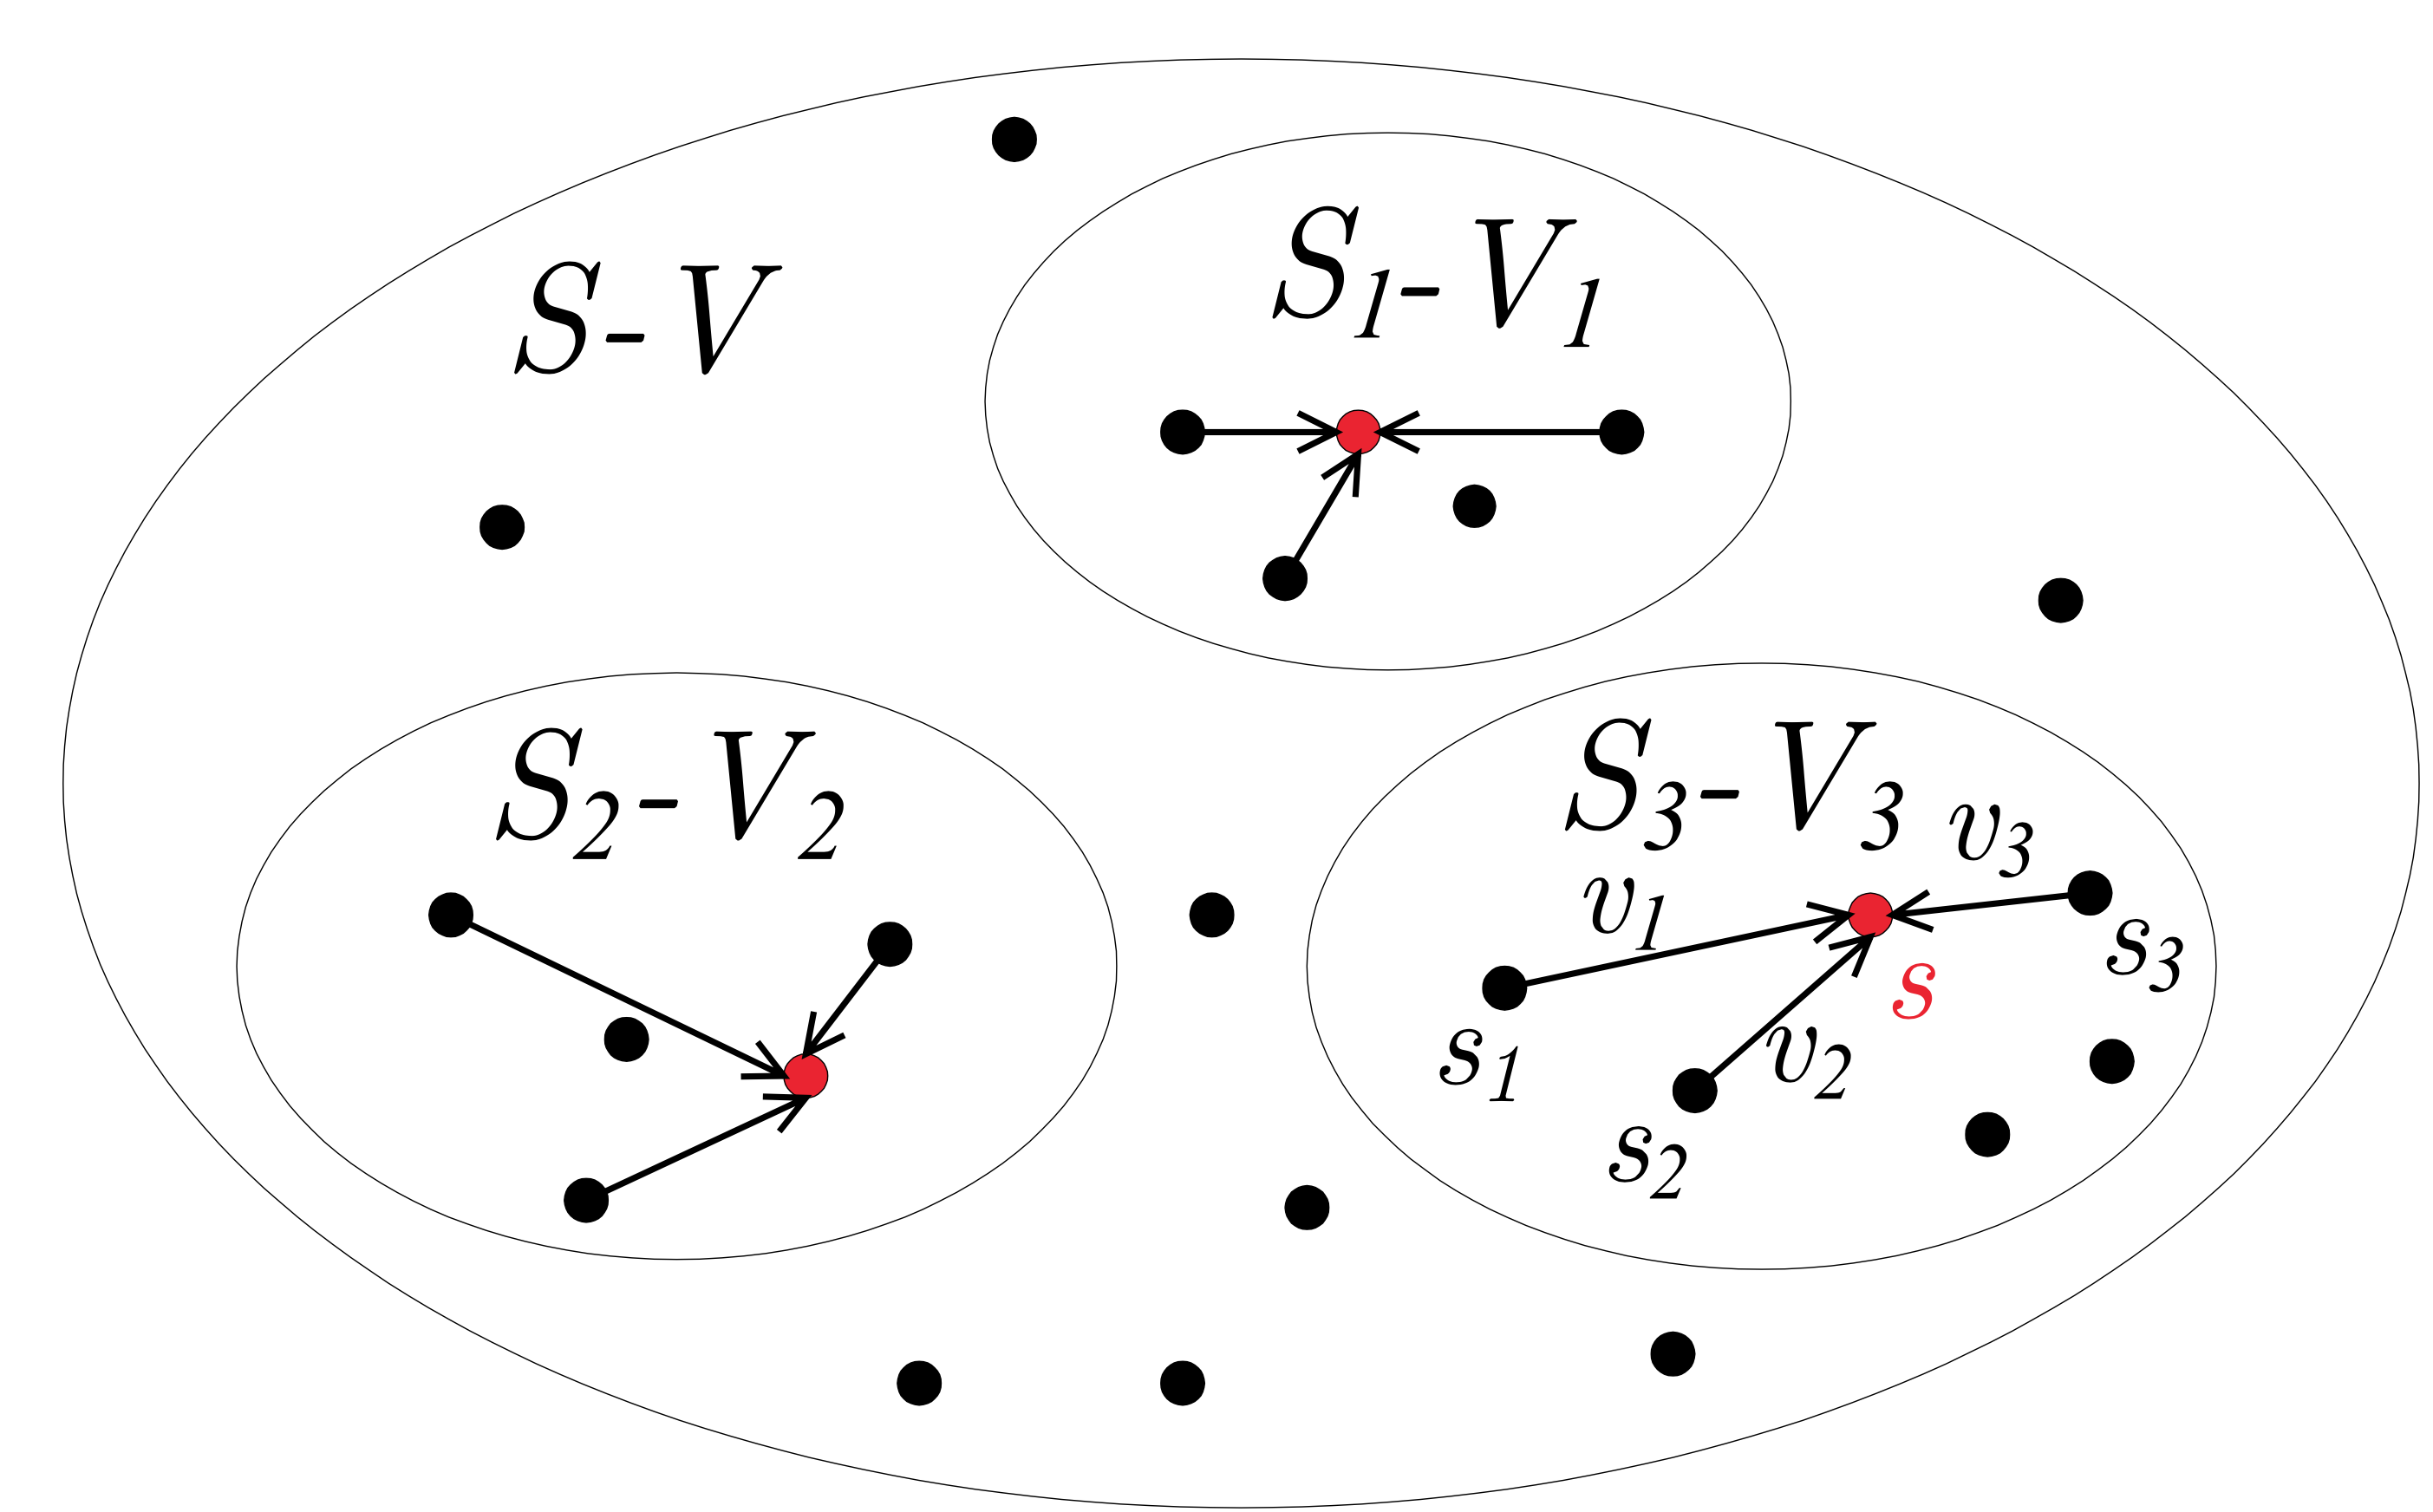
\includegraphics[scale=0.1]{SEL.png}
	\caption{State Space $S$ consists of several subspaces $\{S_1$, $S_2$,..., $S_n\}$, the value function $V$ of a fix point in $S$ defined by combing the value functions $\{V_1, V_2,...,V_n\}$ of each subspace $S_i\ for\ i\in \{1, 2,..., n\}$}
	\label{fig1}
\end{figure}

In OSK-TD, by following this philosophy we divide the whole state space into several subspaces, each subspace can be viewed as a weak learner. Consequently, after combing the kernel-value-weighted prediction of each subspace we would get a better approximated value function with lower generalization error. More generally, the task is to find the optimal local value functions $\{V_1, V_2, ...,V_n\}$ of the subspaces in Fig. 1 and the rule about how to combine them together.\\

As an online TD learning algorithm, the sample dictionary $D_i$ for each subspace $S_i$ should be online dynamically constructed by inserting the feature vectors $\phi$ of samples into $D$ with respect to a kernel selective function $\beta_1(D, \phi)$. Assume, now we have obtained the sparsified dictionary $D$ and the next step is to optimize the parameter vectors $\theta_i$ based on the sample subdictionaries $D_i$ for each subspace $S_i$ so that we improve the generalization ability of the model.\\

Since the sparsified dictionary $D$ consists of several subdictionaries $D_i$, which represent the subspaces $S_i$, where $D=\cup D_i$ and $D_i \cap D_j = \emptyset$ for any $1 \leq i,\ j \leq n$. Therefore, the kernel-based value function can be written in form of $\widetilde{V}(s)=\sum_{i=1}^nV_i(s)$ where
\begin{equation}
	V_i(s) =	\begin{cases}
				\sum_{s_j\in D_t}\theta_j\kappa(s_j, s),& s\in S_i\\
           		0, & \text{otherwise}
      		\end{cases}.
\end{equation}

Selective kernel-based value function can be described as a procedure of selecting  the value functions $V_i \in \{V_1, V_2,..., V_n$\} associated to the corresponding subspace $S_i \in \{S_1, S_2,..., S_n\}$ and summing up them with kernel-distance weights. Similar to the selective function $\beta_1$ used in dictionary based online sparsification, we propose another selective function $\beta_2$ to select the appropriate subset of samples in dictionary $D$ associated to the selected subspaces $S_i \in S$.
\begin{equation}
  \beta_2(s, s_i) =
      \begin{cases}
			1,& s_i \text{\ is appropriate to approximate s}\\
           	0, & \text{otherwise}
      \end{cases},
\end{equation}
where $s\in S, s_i \in D$.

Therefore, after combing the equations we obtain the general form of selective kernel-based value function as follows
\begin{equation}
	\widetilde{V}(s)=\sum_{i=1}^{|D|}\theta_i \beta_2(s, s_i)\kappa(s, s_i), 
\end{equation}
where $|D|$ is the size of the sparsified dictionary $D$.
\subsection{Design of OSK-TD}
In this section, we consider the kernel function choice and at the end OSK-TD is proposed from the algorithmic  perspective.\\

The choice of kernel function plays an important role in kernel-based learning schema. In different problems, algorithms using different kernel functions can  have significantly different behaviours and performances. In OSK-TD the kernel function consists of two parts, the basic kernel function and the selective function. As already proofed in the related work as well as experience, Gaussian kernel function 
\begin{equation}
	\kappa(s, s_{'}) = e^{-\frac{||s-s^{'}||^2}{2\sigma^2}}
\end{equation}
is chosen as the basic kernel function. Recall the kernel distance definition in (49) for the second issue, the kernel distance from the new coming sample $s_t$ to a sample $s_i$ in sparsified dictionary $D$ at time step $t$ is $d(s_i, s_t)=2-2\kappa(s_t, s_i)$ after applying the kernel trick. The kernel-distance based selection function selects exactly the samples in the sparsfied dictionary $D$, which is closer to the new coming sample in RKHS, because the samples far away from coming sample is more likely to be irrelevant and thus possesses a poor representation of value function. Therefore, the selective function can be defined as
\begin{equation}
  \beta_2(s_t, s_i) =
      \begin{cases}
			1,& d(s_t, s_i)\ <\ \mu_2\\
           	0, & \text{otherwise}
      \end{cases}.
\end{equation}

The goal of algorithm is to find a optimal parameter $\Theta^* =\{\theta_1^*, \theta_2^*,...\theta_{|D|}^*\}$, where $|D|$ is the size of sparsified dictionary $|D|$, such that minimize the generalization error in form as
\begin{equation}
	E(\Phi)=\int p(s)\bigg(\sum_{i=1}^{|D|}\theta_i\beta_2(s, s_i)\kappa(s, s_i)-V(s)\bigg)^2,
\end{equation}
where $|D|$ is the size of sparsified dictionary $D$. Gradient method is integrated in OSK-TD und able to decrease the generalization error by updating the parameter vectors in direction of reversal gradient with a step size $\alpha$.\\
\begin{equation}
	\Theta_{t+1} =\Theta_t + \alpha\delta\nabla_{\Theta_t}\widetilde{V}(s_t) ,
\end{equation}
where $\alpha$ is the learning rate, $\delta=r+\gamma \widetilde{V}(s^{'})-\widetilde{V}(s)$, where $\gamma$ is the discount factor, and 
$\nabla_{\Theta_t}={[\beta_2(s, s_i)\kappa(s, s_i)]^{|D|}_{i=1}}^\top$\\

Thus, the elementary update rule of OSK-TD can be derived into form of TD($\lambda$) as follows,
\begin{equation}
	\theta_{i, t+1} = \theta_{i, t}+\alpha \delta_t e_{i, t},
\end{equation}
where $\delta_t = r_{t}+\gamma \widetilde{V}(s_{t+1})-\widetilde{V}(s_t)$, $e_{i, t+1} = \gamma \lambda e_{i, t}+\beta(s, s_t)\kappa(s,s_t)$ and each $\theta_{i, }, e_{i, t}$ is associate with the $i$th row in $\Theta$ at time step $t$.\\

Finally, we give the pseudocode of OSK-TD. Note, because OSK-TD is a prediction version and thus instead of TD($\lambda$) we give the online selective kernel-based TD learning in Q($\lambda$) framework.\\
{
	\removelatexerror% Nullify \@latex@error
	\LinesNumbered
	\begin{algorithm}[H]
		\textup{Initialize parameters($\epsilon, \alpha,\lambda, \mu_1, \mu_2$) and empty sample dictionary $D$}\\

		\Repeat({(for each episode)}){$s$ is terminal}{
	  		$s\leftarrow$ action given by $\pi$ (e.g., $\epsilon$-greedy) for $s$\\
	  		Take action $\alpha$, observe reward $r$, next state $s^{'}$\\
	  		$\delta \leftarrow r+\gamma\widetilde{V}(s^{'})-\widetilde{V}(s)$,\\
	  		\dosemic\nonl where $\widetilde{V}$(s) is computed by (54)\\
  		
  			\Repeat({(for each element $d_i\in D$)}){}{
	  			$s_i, e_i, \theta_i \leftarrow$ get state, eligibility trace and weight associated with $d_i$\\
	  			$e_t\leftarrow \gamma\lambda e_i+\beta(s, s_i)k(s_i, s)$\\
	  			$\theta_i \leftarrow \theta_i + \alpha\delta e_i$
  			}
  			compute the minimum distance according to (55)\\
  			update the sample dictionary $D$ according to (51)\\
  			$s\leftarrow s_{'}$
  		}
 		\caption{OSK-TD}
	\end{algorithm}
}

% needed in second column of first page if using \IEEEpubid{}
%\IEEEpubidadjcol

% An example of a floating figure using the graphicx package.
% Note that \label must occur AFTER (or within) \caption.
% For figures, \caption should occur after the \includegraphics.
% Note that IEEEtran v1.7 and later has special internal code that
% is designed to preserve the operation of \label within \caption
% even when the captionsoff option is in effect. However, because
% of issues like this, it may be the safest practice to put all your
% \label just after \caption rather than within \caption{}.
%
% Reminder: the "draftcls" or "draftclsnofoot", not "draft", class
% option should be used if it is desired that the figures are to be
% displayed while in draft mode.
%
%\begin{figure}[!t]
%\centering
%\includegraphics[width=2.5in]{myfigure}
% where an .eps filename suffix will be assumed under latex, 
% and a .pdf suffix will be assumed for pdflatex; or what has been declared
% via \DeclareGraphicsExtensions.
%\caption{Simulation Results}
%\label{fig_sim}
%\end{figure}

% Note that IEEE typically puts floats only at the top, even when this
% results in a large percentage of a column being occupied by floats.


% An example of a double column floating figure using two subfigures.
% (The subfig.sty package must be loaded for this to work.)
% The subfigure \label commands are set within each subfloat command, the
% \label for the overall figure must come after \caption.
% \hfil must be used as a separator to get equal spacing.
% The subfigure.sty package works much the same way, except \subfigure is
% used instead of \subfloat.
%
%\begin{figure*}[!t]
%\centerline{\subfloat[Case I]\includegraphics[width=2.5in]{subfigcase1}%
%\label{fig_first_case}}
%\hfil
%\subfloat[Case II]{\includegraphics[width=2.5in]{subfigcase2}%
%\label{fig_second_case}}}
%\caption{Simulation results}
%\label{fig_sim}
%\end{figure*}
%
% Note that often IEEE papers with subfigures do not employ subfigure
% captions (using the optional argument to \subfloat), but instead will
% reference/describe all of them (a), (b), etc., within the main caption.


% An example of a floating table. Note that, for IEEE style tables, the 
% \caption command should come BEFORE the table. Table text will default to
% \footnotesize as IEEE normally uses this smaller font for tables.
% The \label must come after \caption as always.
%
%\begin{table}[!t]
%% increase table row spacing, adjust to taste
%\renewcommand{\arraystretch}{1.3}
% if using array.sty, it might be a good idea to tweak the value of
% \extrarowheight as needed to properly center the text within the cells
%\caption{An Example of a Table}
%\label{table_example}
%\centering
%% Some packages, such as MDW tools, offer better commands for making tables
%% than the plain LaTeX2e tabular which is used here.
%\begin{tabular}{|c||c|}
%\hline
%One & Two\\
%\hline
%Three & Four\\
%\hline
%\end{tabular}
%\end{table}


% Note that IEEE does not put floats in the very first column - or typically
% anywhere on the first page for that matter. Also, in-text middle ("here")
% positioning is not used. Most IEEE journals use top floats exclusively.
% Note that, LaTeX2e, unlike IEEE journals, places footnotes above bottom
% floats. This can be corrected via the \fnbelowfloat command of the
% stfloats package.


\section{Experiment}
In this paper, two experiments are used to demonstrate the effectiveness of the three algorithms on the continuous reinforcement learning problems: Mountain Car and Cart Pole. Theses two standard Reinforcement Learning benchmarks in the NIPS Workshop 2005 are two traditinal RL problems and also used to evaluate various of reinforcement learning algorithms. Note, because OSK-TD is a prediction algorithm. We combine OSK-TD with Q-learning to learn for the control task in the two experiments.\\

The proposed algorithms' performance will be evaluated for their convergence, running time and sparsity with varied learning parameters. The same predefined parameters for each experiment are: 1. The curves are generated  by averaging the sum of rewards for 20 runs. 2. the discount factor is 0.9. 3) An episode is limited to 1000 steps.
\subsection{Mountain Car}
In Mountain Car simulation \cite{sutton1998reinforcement}, the learning agent needs to drive an underpowered car upon a sttep mountain road. The reward for each step is -1 until the car has reached its goal position on the top of mountain and the episode ends. There are three possible actions, full throttle forward (+1), full throttle backward (-1) and zero throttle (0). The car movement is based on the simple system dynamics, where position of the car is $x_t$ and velocity is $\dot{x_t}$. And the they are bounded by the simulator at $-2.4 \leq x_{t+1} \leq 2.4$ and $-0.20943951 \leq \dot{x}_{t+1} \leq 0.20943951$. The simulation starts at position $x_0=-0.3$ and the goal position $x_T=0.5$.\\

1. The OSK-Q algorithm fails unfortunately, it is not able to learn from the simulation even after a fine parameter tunning, we can see The main reason maybe lack of convergence of non-linear value function approximation, which was mentioned in \cite{tsitsiklis1997analysis}. However, from the learning curve in Fig.2, we can see GQ($\lambda$) ane Ro-GQ($\lambda$) have successfully learned the policies from the experiment. 2. GQ($\lambda$) works more stablely and faster than the RO-GQ($\lambda$). 3. RO-GQ($\lambda$) is more sensitive to the parameter setting, especially $\lambda$ and regularization factor. 4. The higher regularization factor is, the more sparse will the action-value function and more unstable the algorithm will be.
\subsection{Cart Pole}
In Cart Pole simulations \cite{sutton1998reinforcement}, the learning agent needs to actively balance an unstable inverted pendulum mounted on a cart and keep it upright by moving the the cart horizontally. The reward for each step is 1 and 0 when the inverted pendulum fells (episode terminated), the goal of the experient is to keey the inverted pendulum upright as long as possible. Two possible actions are move left (-1) or right (+1) and the action has only freedom one. The system dynamics of Cart Pole is highly non-linear and more complicated than Mountain Car. The parameters are the position of cart $x_t$, the velocity of cart $\dot{x}_t$, the angle of pole $\theta_t$ and the rotation rate of pole $\dot{\theta}_t$. The are also bounded by the simulator at $-1.2 \leq x_{t+1} \leq 0.5$ and $-0.07 \leq \dot{x}_{t+1} \leq0.07$.
\section{Conclusion}
In this paper, three learning algorithms were proposed to deal with large scale and continuous RL problems. GQ($\lambda$) and RO-GQ($\lambda$) are traditional tabular-form learning algorithm while OSKTD is a selective kernel-based learning algorithm. For sparsification, different approaches have been applied. RO-GQ($\lambda$) generate the sparsity by minimizing a cost function with a $\ell1$ norm regularization term while OSK-Q follows a online kernel sparsification procedure.\\

GQ($\lambda$)


% if have a single appendix:
%\appendix[Proof of the Zonklar Equations]
% or
%\appendix  % for no appendix heading
% do not use \section anymore after \appendix, only \section*
% is possibly needed

% use appendices with more than one appendix
% then use \section to start each appendix
% you must declare a \section before using any
% \subsection or using \label (\appendices by itself
% starts a section numbered zero.)
%

  
%\appendices
%\section{Proof of the First Zonklar Equation}

% use section* for acknowledgement
%\section*{Acknowledgment}


%The authors would like to thank..


% Can use something like this to put references on a page
% by themselves when using endfloat and the captionsoff option.
% \ifCLASSOPTIONcaptionsoff
%   \newpage
% \fi


\newpage
% trigger a \newpage just before the given reference
% number - used to balance the columns on the last page
% adjust value as needed - may need to be readjusted if
% the document is modified later
%\IEEEtriggeratref{8}
% The "triggered" command can be changed if desired:
%\IEEEtriggercmd{\enlargethispage{-5in}}

% references section

% can use a bibliography generated by BibTeX as a .bbl file
% BibTeX documentation can be easily obtained at:
% http://www.ctan.org/tex-archive/biblio/bibtex/contrib/doc/
% The IEEEtran BibTeX style support page is at:
% http://www.michaelshell.org/tex/ieeetran/bibtex/
%\bibliographystyle{IEEEtran}
% argument is your BibTeX string definitions and bibliography database(s)
%\bibliography{IEEEabrv,../bib/paper}
%
% <OR> manually copy in the resultant .bbl file
% set second argument of \begin to the number of references
% (used to reserve space for the reference number labels box)
\bibliographystyle{IEEEtran}
\bibliography{IEEEabrv,reference}

% \begin{thebibliography}{1}
% \bibitem{Reinforcement learning: An introduction}
% R. S. Sutton and A. G. Barto, \emph{Reinforcement learning: An introduction}, 2nd~ed. \hskip 1em plus
%   0.5em minus 0.4em\relax Cambridge, MA: MIT Press, 1998.
% \bibitem{An analysis of temporal-difference learning with function approximation}
% J. N. Tsitsiklis and B. Van Roy, "An analysis of temporal-difference learning with function approximation," in \emph{IEEE Transactions on Automatic Control}, vol. 42, no. 5, pp. 674–690, May 1997.
% \bibitem{An analysis of linear models, linear value-function approximation, and feature selection for reinforcement learning}
% R. Parr, L. Li, G. Taylor, C. Painter-Wakefield, and M. L. Littman, “An analysis of linear models, linear value-function approximation, and feature selection for reinforcement learning,” in \emph{Proceedings of the 25th international conference on Machine learning}, Helsinki, Finland, Jul. 2008, pp. 752-759.
% \bibitem{Tree-based batch mode reinforcement learning.}
% Ernst, Damien, Pierre Geurts, and Louis Wehenkel, "Tree-based batch mode reinforcement learning," in Journal of Machine Learning Research 6.Apr (2005): 503-556. 
% \end{thebibliography}

% biography section
% 
% If you have an EPS/PDF photo (graphicx package needed) extra braces are
% needed around the contents of the optional argument to biography to prevent
% the LaTeX parser from getting confused when it sees the complicated
% \includegraphics command within an optional argument. (You could create
% your own custom macro containing the \includegraphics command to make things
% simpler here.)
%\begin{biography}[{\includegraphics[width=1in,height=1.25in,clip,keepaspectratio]{mshell}}]{Michael Shell}
% or if you just want to reserve a space for a photo:

% \begin{IEEEbiography}[{\includegraphics[width=1in,height=1.25in,clip,keepaspectratio]{picture}}]{John Doe}
% % \blindtext
% [1] R. S. Sutton and A. G. Barto, Reinforcement learning: An introduction, 2nd ed. Cambridge, MA: MIT Press, 1998.
% \end{IEEEbiography}

% You can push biographies down or up by placing
% a \vfill before or after them. The appropriate
% use of \vfill depends on what kind of text is
% on the last page and whether or not the columns
% are being equalized.

%\vfill

% Can be used to pull up biographies so that the bottom of the last one
% is flush with the other column.
%\enlargethispage{-5in}




% that's all folks
\end{document}


